% Primarily this section should be about scientific methods and theories you need to evaluate/compare/invent to solve your problems from 1.3.
% In some cases it may be ok to describe different technologies, but the purpose is to describe something and then draw a conclusion from that.
% Example, if you decide to discuss different databases, it may be for the purpose of selecting the best type for your implementation later on (based on for example data representation, scalability, speed, etc.).
% Optimally the problems in 1.3 are not solved by anyone else yet, in which case this section needs to describe how to solve them (new algorithms, mathematical approaches, etc.).
 
% This section can have a lot of subsections (3.1, 3.2, 3.3, etc).

% TODO: Explain Unwinding call stack

To virtually unwind the \emph{call stack} entail the task of restoring the code location and the register values for each \emph{subroutine activation}.
It also entail the task of find the location of the corresponding \emph{call frame} on the stack for each \emph{subroutine activation}.


Each \emph{subroutine activation} has a code location within the subroutine, it describes where it stopped.
The reason for stopping could be that a breakpoint was hit, it was interrupted by a event or it could be location were it made a call to the next subroutine.
A activation also describe the state of some of the registers where it stopped.
These are the registers that need to be preservd during the call to another subroutine.
They can be restored by virtualy unwidning using the information stored in \gls{DWARF} section \emph{.debug\_frame}.
Lastly a activation is identified by its \gls{cfa} value. 
The \gls{cfa} is the value of the stack pointer in the previous stack frame for the stopped code location of the activation.
One thing to note is that the \gls{cfa} is not the same value as the stack pointer when entering the current \emph{call frame}(see \cite{dwarf} page 126).


Accessing one of the \emph{subroutine activation} requires that the activation stack is virtually unwind to get to the desired activation, there is only one exception to this and that is if the top activation is desired.
That is because all of \emph{activation} information location is known thus it is easy to read that information from the registers and memory. 
It is called \emph{virtually unwinding} because none of the value in the registers or memory are changes which means that the state of the target is not changed.
In general the steps to virtually unwinding the \emph{activation} is to begin with calculating the \gls{cfa} of the previous \emph{activation}, the code location of the previous \emph{activation} and to virtually restore any registers if needed.
Then the same thing can be done to the previous \emph{activation} and so it repeats until the desired \emph{activation} is reached.
This process is required to start with the top \emph{activation} because it is the only one that is known at first and the process has to be stopped if the bottom \emph{activation} is reached.


Any subroutine can have some prologue code that is in the beginning of the subroutine  and epilogue code that is at the end.
The prologue code is used to preserve the values of registers over the duration of the subroutine, this is done by allocating some extra space on the call stack for the \emph{call frame} which is used to store the register values.
Then the epilogue code is used to restore these values to the registers before returning to the previous frame.
Using this fact the compiler generates debug information that enables a user to virtually restore these preserved registers and that is what is done when virtually unwinding the \emph{activations}.
One thing to note is that the prologue and epilogue code are not always continues blocks of code that are in the beginning and end of a subroutine.
Instead sometimes the store and read operation are moved into the subroutine.
There more of these special cases that the compiler does and some that are hardware specific, to read more about them see \cite{dwarf} page 126-127.


The location information for finding \gls{cfa} and the registers for a \emph{activation} is stored in a table, that consist of virtual unwinding rules and addresses.
There are multiple of these tables for each frame that are stored in a data structure called \gls{fde} that is meant to hold all the needed frame information for that frame.
Then there is also the data structure \gls{cie} that holds information that is shared between some \acrlong{fde}'s.
All of this frame information is stored in a separate section called \emph{.debug\_frame} and each instance of this section is guaranteed to have at least one \acrlong{cie}.


Going back to the table with the virtual unwinding rules the first column of that table contains the code addresses, they are used to identify that all the virtual unwinding rules on that row applies for a particular code address.
Every line of code is meant to have these rules but because many of the rows are exactly the same many of those rows are removed from the table to save storage space.
The second column is also special because it contains the virtual unwinding rules for \gls{cfa}, these rules are either a \gls{DWARF} expression that needs to be evaluated in the same way that the variables are in section \ref{sec:evaluate-variable} or a register values plus some singed offset.
All the other columns contain virtual unwinding rules for all the register and they are in orders from $0$ to $n$, see figure \ref{fig:stacktracetable} for a visual example of the table.


\begin{figure}[h]
	\centering
	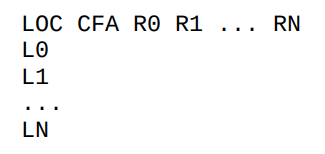
\includegraphics[width=0.5\textwidth]{stacktrace-table.png}
	\caption{This is how the table for reconstructing the \gls{cfa} and registers looks like. \emph{LOC} means that it is the column containing the code locations for $0$ to $N$. The column with \gls{cfa} has the virtual unwinding rules for \gls{cfa}. The rest of the column \emph{R0} to \emph{RN} holds all the virtual unwinding rules for the register $0$ to $N$.}
	\label{fig:stacktracetable}
\end{figure}


There are a number of different virtual unwinding rules for the registers that are called register rules in the \gls{DWARF} specification \cite{dwarf}, these are listed on page 128.
Some of them are very easy to use such as the register rule \emph{undefined} that says that a register is not preserved by the callee and thus is impossible to know the value of.
If the register value is unchanged then register rule \emph{same value} is used to denote that.
The must common rule is \emph{offset(N)} where \emph{N} is a signed offset, this rule means that the register value is stored at the address $\gls{cfa}+N$.
All of the remaining rules can be read about in the \gls{DWARF} specification \cite{dwarf} on page 128.


Now understanding what information is stored about the call frames the call stack can be virtually unwind by first finding the relevant \gls{cie} and \gls{fde}.
Finding the relevant \gls{cie} and \gls{fde} is done by doing a lookup in the \gls{DWARF} section \emph{.debug\_frame} using the current machine code location that the program is stopped on.
Then the virtual unwinding rules in the table of the \gls{fde} can be evaluated to get the value of the \gls{cfa} and the preserved register.
Lastly the code location of the previous frame can be calculated using the return register that is must often one of the preserved registers, this can not always be done because sometimes the information needed is not present.
The most common case were the value of the return register is not preserved is when the bottom of the stack is reach, thus the virtual unwinding is complete.
This way of virtually unwind a \emph{activation} can then be repeat for all the actiavations in the stack starting from the top \emph{activation} of the stack to the bottom one.


The virtual unwinding rules in the table actually needs to be evaluated from some special \gls{DWARF} operations.
There are a lot of these operation which many are similar to the operation used to evaluate the location of a value in section \ref{sec:evaluate-variable}.
Thus there is no real need of explain them here but to learn more about them read section $6.4.2$ in the \gls{DWARF} specification \cite{dwarf} on pages 131-136.
The way to evaluate these operations is also describe in section $6.4.3$ in the \gls{DWARF} specification \cite{dwarf} on pages 136-137 in $4$ steps.

